% !TeX program = xelatex
% 单文件 Beamer 课件，无外置主题、图片或字体文件依赖。
% 编译：在本目录运行 xelatex -interaction=nonstopmode "main.tex" 两次。
% 在下一行取消注释，可另行编译出每张幻灯片后附教师备注的版本。
% \def\TeacherNotes{1}
\documentclass[aspectratio=169,10pt]{beamer}
\usepackage[UTF8,fontset=fandol]{ctex}
\IfFontExistsTF{Microsoft YaHei}{\setCJKsansfont{Microsoft YaHei}}{}
\usepackage{amsmath,amssymb,tikz}
\usetikzlibrary{calc,angles,quotes,arrows.meta}
\definecolor{campusgreen}{HTML}{126831}
\definecolor{ink}{HTML}{183025}
\definecolor{muted}{HTML}{63756B}
\definecolor{warm}{HTML}{A65A1F}
\definecolor{errorred}{HTML}{AB3838}
\setbeamercolor{normal text}{fg=ink,bg=white}
\setbeamercolor{structure}{fg=campusgreen}
\setbeamercolor{frametitle}{fg=campusgreen,bg=white}
\setbeamerfont{normal text}{size=\fontsize{12}{18}\selectfont}
\setbeamerfont{frametitle}{size=\fontsize{16}{21}\selectfont,series=\bfseries}
\setbeamersize{text margin left=8mm,text margin right=8mm}
\setbeamertemplate{navigation symbols}{}
\setbeamertemplate{headline}{}
\setbeamertemplate{frametitle}{\vspace*{3mm}\insertframetitle\par\vspace*{3mm}}
\newcommand{\LessonTime}{00:00--00:30}
\newcommand{\settime}[1]{\gdef\LessonTime{#1}}
\setbeamertemplate{footline}{%
  \hspace*{8mm}{\color{muted}\fontsize{7}{9}\selectfont\LessonTime\quad 分钟}%
  \hfill{\color{muted}\fontsize{7}{9}\selectfont\insertframenumber/\inserttotalframenumber}\hspace*{8mm}\vspace*{3mm}}
\ifdefined\TeacherNotes
  \setbeameroption{show notes}
\else
  \setbeameroption{hide notes}
\fi
\newcommand{\key}[1]{{\color{campusgreen}\bfseries #1}}
\newcommand{\bigmath}[1]{\begingroup\color{campusgreen}\fontsize{18}{25}\selectfont\[#1\]\endgroup}
\newcommand{\gap}{\par\vspace{4mm}}
\newcommand{\vcaref}{Needham，\textit{Visual Complex Analysis}，25周年版（2023），第1章\S1.3.3，第18--22页。}

% 主构型由明确坐标独立重绘，非书中图像截图。
% A=0，B=4+i，C=3-3i，ABC顺时针。
% 左侧正方形中心p=(3+5i)/2，右侧中心s=-3i，m=(7-2i)/2。
% 因而p-m=-2+3.5i，s-m=-3.5-2i=i(p-m)。
\newcommand{\trianglefigure}[1]{%
\begin{tikzpicture}[x=.42cm,y=.42cm,font=\scriptsize,>=Stealth]
  \path[use as bounding box] (-3.7,-6.8) rectangle (5.1,5.8);
  \coordinate(A)at(0,0);\coordinate(B)at(4,1);\coordinate(C)at(3,-3);
  \coordinate(P)at(1.5,2.5);\coordinate(S)at(0,-3);\coordinate(M)at(3.5,-1);
  \filldraw[draw=campusgreen!70,fill=campusgreen!7] (A)--(B)--(3,5)--(-1,4)--cycle;
  \filldraw[draw=campusgreen!70,fill=campusgreen!7] (A)--(C)--(0,-6)--(-3,-3)--cycle;
  \draw[thick,ink] (A)--(B)--(C)--cycle;
  \draw[very thick,campusgreen] (M)--(P);
  \draw[very thick,warm] (M)--(S);
  \pic[draw=ink,angle radius=3mm] {right angle=P--M--S};
  \foreach\v in {A,B,C,P,S,M}{\fill[ink](\v)circle(1.5pt);}
  \ifnum#1=1
    \node[left]at(A){$A(0)$};\node[right]at(B){$B(b)$};\node[below right]at(C){$C(c)$};
  \else
    \node[left]at(A){$A$};\node[right]at(B){$B$};\node[below right]at(C){$C$};
  \fi
  \node[above left]at(P){$P(p)$};\node[below left]at(S){$S(s)$};\node[right]at(M){$M(m)$};
\end{tikzpicture}}

\newcommand{\centerfigure}{%
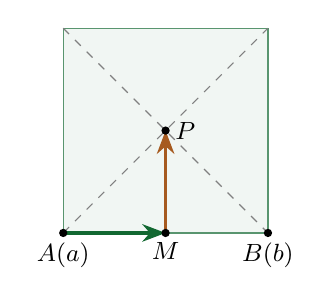
\begin{tikzpicture}[x=.65cm,y=.65cm,font=\small,>=Stealth]
  \filldraw[draw=campusgreen!70,fill=campusgreen!6] (0,0)rectangle(4,4);
  \draw[gray,dashed](0,0)--(4,4)(0,4)--(4,0);
  \draw[very thick,->,campusgreen](0,0)--(2,0);
  \draw[very thick,->,warm](2,0)--(2,2);
  \fill(0,0)circle(1.5pt)node[below]{$A(a)$};
  \fill(4,0)circle(1.5pt)node[below]{$B(b)$};
  \fill(2,0)circle(1.5pt)node[below]{$M$};
  \fill(2,2)circle(1.5pt)node[right]{$P$};
\end{tikzpicture}}

\newcommand{\rotationfigure}{%
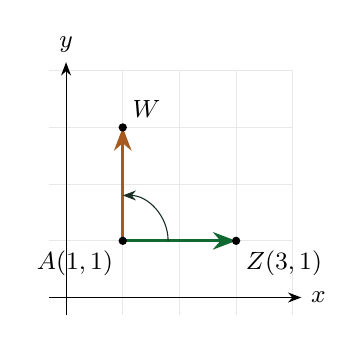
\begin{tikzpicture}[x=.72cm,y=.72cm,font=\small,>=Stealth]
  \draw[step=1,gray!18](-.3,-.3)grid(4,4);
  \draw[->](-.3,0)--(4.15,0)node[right]{$x$};\draw[->](0,-.3)--(0,4.15)node[above]{$y$};
  \coordinate(A)at(1,1);\coordinate(Z)at(3,1);\coordinate(W)at(1,3);
  \draw[very thick,->,campusgreen](A)--(Z);
  \draw[very thick,->,warm](A)--(W);
  \draw[->,ink](1.8,1)arc(0:90:.8);
  \fill(A)circle(1.5pt)node[below left]{$A(1,1)$};
  \fill(Z)circle(1.5pt)node[below right]{$Z(3,1)$};
  \fill(W)circle(1.5pt)node[above right]{$W$};
\end{tikzpicture}}

% 凸四边形ABCD逆时针；四个正方形均向外。
\newcommand{\quadrifigure}{%
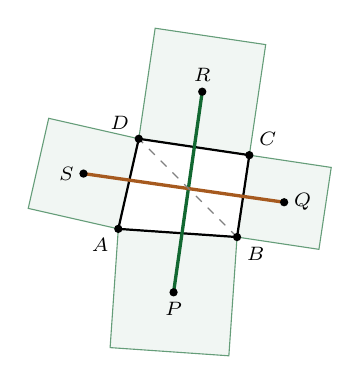
\begin{tikzpicture}[x=.52cm,y=.52cm,font=\scriptsize]
  \coordinate(A)at(-1.5,-.8);\coordinate(B)at(1.4,-1);
  \coordinate(C)at(1.7,1);\coordinate(D)at(-1,1.4);
  \filldraw[draw=campusgreen!65,fill=campusgreen!6](A)--(B)--(1.2,-3.9)--(-1.7,-3.7)--cycle;
  \filldraw[draw=campusgreen!65,fill=campusgreen!6](B)--(C)--(3.7,.7)--(3.4,-1.3)--cycle;
  \filldraw[draw=campusgreen!65,fill=campusgreen!6](C)--(D)--(-.6,4.1)--(2.1,3.7)--cycle;
  \filldraw[draw=campusgreen!65,fill=campusgreen!6](D)--(A)--(-3.7,-.3)--(-3.2,1.9)--cycle;
  \draw[thick](A)--(B)--(C)--(D)--cycle;
  \coordinate(P)at(-.15,-2.35);\coordinate(Q)at(2.55,-.15);
  \coordinate(R)at(.55,2.55);\coordinate(S)at(-2.35,.55);
  \draw[very thick,campusgreen](P)--(R);\draw[very thick,warm](Q)--(S);
  \draw[gray,dashed](B)--(D);
  \foreach\v/\pos in {A/below left,B/below right,C/above right,D/above left,P/below,Q/right,R/above,S/left}{\fill(\v)circle(1.5pt)node[\pos]{$\v$};}
\end{tikzpicture}}

\begin{document}
\usebeamerfont{normal text}

\settime{00:00--00:30}
\begin{frame}[plain]
\vspace{11mm}
{\color{campusgreen}\bfseries\fontsize{25}{32}\selectfont 复数破解平面几何\par}
\vspace{8mm}
{\fontsize{17}{23}\selectfont 两个正方形，藏着什么关系？\par}
\vspace{13mm}
AI伴学·第3课时\qquad 华光辉\par\vspace{4mm}45分钟\hfill\textcolor{muted}{几何探索课}
\note{本课以几何问题为主体。上次用乘i描述直角旋转，今天把这一动作与位移、中点组合起来，解释一个对任意三角形都成立的关系。}
\end{frame}

\settime{00:30--04:00}
\begin{frame}[t]{任意三角形中的一个意外关系}
\begin{columns}[c,onlytextwidth]
\column{.36\textwidth}\centering\trianglefigure{0}
\column{.61\textwidth}
在三角形$ABC$的两边$AB,AC$\par 外侧分别作正方形。
\gap 中心为$P,S$，$M$为$BC$中点。
\bigmath{MP=MS,\qquad MP\perp MS}
为什么三角形怎样变化，\par 这个关系都成立？
\end{columns}
\note{先读非退化三角形、外侧、中心、中点等条件。图中已标直角，任务是解释为什么必然成立，不作盲测猜想。让学生纸笔尝试1分钟。这类问题有初等解法，本课展示复数的统一表达。依据：\vcaref 图1.12b。图形按自选坐标独立重绘。}
\end{frame}

\settime{04:00--07:00}
\begin{frame}[t]{几何中的一段路，用复数相减}
点$A,B$对应复数$a,b$。从$A$到$B$的位移是
\bigmath{b-a.}
例如：
\[(4+3i)-(1+i)=3+2i.\]
\gap 点的位置，与从一个点走到另一个点的位移不同。
\gap\key{比较两条线段的方向，先把它们写成位移。}
\note{终点减起点，不能写反。例子解释为向右3、向上2。不要求额外掌握向量公理。}
\end{frame}

\settime{07:00--10:00}
\begin{frame}[t]{旋转中心换了，先减再加}
以点$A(a)$为中心，将点$Z(z)$逆时针旋转$90^\circ$：
\bigmath{w=a+i(z-a).}
\gap $z-a$：从中心出发的位移。
\gap $i(z-a)$：将这段位移逆时针旋转$90^\circ$。
\gap\key{再加$a$：得到终点的位置。}
\note{iz只表示绕原点的旋转。先将中心平移到原点，旋转后再平移回来。依据原书第20页的旋转分解，只取直角旋转，不引入欧拉公式。}
\end{frame}

\settime{10:00--12:00}
\begin{frame}[t]{小检查：中心不是原点}
\begin{columns}[c,onlytextwidth]
\column{.38\textwidth}\centering\rotationfigure
\column{.59\textwidth}
以$A(1,1)$为中心，\par 将$Z(3,1)$逆时针旋转$90^\circ$。
\gap 先在纸上判断终点，\par 再写复数算式。
\[a=1+i,\qquad z=3+i.\]
\key{最后有没有加回中心的位置？}
\end{columns}
\note{目标：区别位置与位移；难度基础。独立1分钟后核对：w=1+3i，对应(1,3)。先减中心与最后加回中心各1分。错用iz会得到(-1,3)。图中W提示方向但未给出坐标答案，应要求解释计算。}
\end{frame}

\settime{12:00--16:00}
\begin{frame}[t]{一个正方形的中心怎样表示}
\begin{columns}[c,onlytextwidth]
\column{.34\textwidth}\centering\centerfigure
\column{.63\textwidth}
沿有向边$AB$，先到中点，\par 再向侧面走半条边。
\[\text{边的中点：}\quad\frac{a+b}{2}.\]
\[\text{左侧中心：}\quad\frac{a+b}{2}+i\frac{b-a}{2}.\]
\[\text{右侧中心：}\quad\frac{a+b}{2}-i\frac{b-a}{2}.\]
\end{columns}
\note{半条边旋转90度恰是边中点到正方形中心的位移。左右侧相对于有向边，不是屏幕上方、下方。图示左侧情形，右侧同理。让学生解释式中的每一项。}
\end{frame}

\settime{16:00--18:00}
\begin{frame}[t]{主问题：把公共顶点取为原点}
\begin{columns}[c,onlytextwidth]
\column{.36\textwidth}\centering\trianglefigure{1}
\column{.61\textwidth}
$A$取为原点，$B,C$对应$b,c$。
\gap $A,B,C$按\key{顺时针}排列。
\gap $AB$外接正方形中心对应$p$。
\gap $AC$外接正方形中心对应$s$。
\gap $BC$中点对应$m$。
\end{columns}
\note{改变原点不改变长度和夹角，不损失一般性。ABC顺时针，AB外侧在有向AB左侧，AC外侧在有向AC右侧。大写P,S,M表示点，小写p,s,m表示相应复数。}
\end{frame}

\settime{18:00--20:00}
\begin{frame}[t]{第一个中心：半条边，再转直角}
\begin{columns}[c,onlytextwidth]
\column{.36\textwidth}\centering\trianglefigure{1}
\column{.61\textwidth}
$AB$外侧在有向边$AB$左侧。
\bigmath{p=\frac b2+i\frac b2}
\bigmath{p=\frac{b+ib}{2}}
\key{先到中点，再向外侧走。}
\end{columns}
\note{让学生分别说明两个加数。若三角形顶点顺序改变，旋转符号必须同步改变。}
\end{frame}

\settime{20:00--22:00}
\begin{frame}[t]{第二个中心：这次向右转}
\begin{columns}[c,onlytextwidth]
\column{.36\textwidth}\centering\trianglefigure{1}
\column{.61\textwidth}
$AC$外侧在有向边$AC$右侧。
\bigmath{s=\frac c2-i\frac c2}
\bigmath{s=\frac{c-ic}{2}}
\textcolor{warm}{顺时针$90^\circ$，对应乘$-i$。}
\end{columns}
\note{目标为方向表达，难度中等。若两个中心都取+i，要求沿有向AC观察外侧。可用-i乘1得到-i，核对顺时针方向。}
\end{frame}

\settime{22:00--23:00}
\begin{frame}[t]{第三边的中点，只需要平均数}
\bigmath{p=\frac{b+ib}{2},\qquad s=\frac{c-ic}{2}}
\vspace{3mm}
\bigmath{m=\frac{b+c}{2}}
\gap\key{中点：横坐标取平均，纵坐标也取平均。}
\note{让学生把三个表达式放在同一张纸上。下一步比较的不是p与s，而是从m出发的两段位移。}
\end{frame}

\settime{23:00--25:00}
\begin{frame}[t]{等长且垂直，合成一个目标}
从$M$到$P$：$p-m$；\qquad 从$M$到$S$：$s-m$。
\bigmath{s-m=i(p-m)}
\gap 如果这个等式成立，就同时得到：
\bigmath{MP=MS,\qquad MP\perp MS.}
\note{位移乘i保持长度并逆时针旋转90度。旋转中心是M，不能写成s=ip。非退化三角形与外侧构造保证两段位移非零。}
\end{frame}

\settime{25:00--28:00}
\begin{frame}[t]{两段位移之间的直角旋转}
\begin{align*}
2(p-m)&=ib-c,\\[4mm]
2(s-m)&=-b-ic.
\end{align*}
\bigmath{i(ib-c)=i^2b-ic=-b-ic}
\gap 同一个表达式出现了：\key{$s-m=i(p-m)$}。
\note{先让学生独立化简p-m，再展示另一式。只需分配律、i平方等于负1。易错为i平方乘b写成正b。不要转而分别求长度和斜率。}
\end{frame}

\settime{28:00--30:00}
\begin{frame}[t]{一个等式，解释两个几何结论}
\begin{columns}[c,onlytextwidth]
\column{.36\textwidth}\centering\trianglefigure{0}
\column{.61\textwidth}
\bigmath{s-m=i(p-m)}
以$M$为中心，\par $P$逆时针旋转$90^\circ$后到$S$。
\gap\key{$MP=MS$，且$MP\perp MS$。}
\gap 除方向、非退化的条件外，\par 推导没有限定$b,c$的具体数值。
\end{columns}
\note{让学生用完整的一句话复述，必须说出旋转中心M。回到原图而非只停留在算式。原书图1.12b提供问题，本课采用自行选择原点的直接代数证明。}
\end{frame}

\settime{30:00--33:00}
\begin{frame}[t]{换一组数，检验你能否使用它}
\bigmath{A:0,\qquad B:4+2i,\qquad C:6-2i}
仍在$AB,AC$外侧作正方形，中心对应$p,s$。
\gap （1）求$p,s$，以及$BC$的中点$m$。
\gap （2）计算$p-m,s-m$，检查旋转关系。
\note{自编中等题，ABC顺时针。答案p=1+3i，s=2-4i，m=5。位移为-4+3i、-3-4i。三个位置各1分，位移与关系各1分，共5分。基础支持只先算p。一组数据不能替代一般证明。}
\end{frame}

\settime{33:00--34:00}
\begin{frame}[t]{核对：两条位移互相检查}
\[p=1+3i,\qquad s=2-4i,\qquad m=5.\]
\bigmath{p-m=-4+3i}
\bigmath{s-m=-3-4i=i(-4+3i)}
算对一个例子，不能代替所有情况的一般证明。
\note{两线段长度均为5。长度核验只能检查部分运算，解释垂直的是乘i关系。保留原始步骤，定位最早不同的等号。}
\end{frame}

\settime{34:00--36:00}
\begin{frame}[t]{请AI查错：漏掉的是什么}
\textcolor{muted}{\small 课堂自编错误样例}
\gap\textcolor{errorred}{“以$M$为中心，逆时针旋转$90^\circ$，所以$s=ip$。”}
\gap 给AI的请求：
\gap\key{“先问我一个关于旋转中心的问题，\par 帮助我检查这句话，不直接给完整证明。”}
\gap 核验依据：这里应比较点的位置，还是两段位移？
\note{正确关系s-m=i(p-m)。本页不冒充真实AI回答。教师仅输入匿名样例，最多等30秒，无网则教师问：i乘的是点的位置，还是从M出发的位移？不上传学生身份信息或整本教材。}
\end{frame}

\settime{36:00--39:00}
\begin{frame}[t]{独立迁移：这次不看AI和例题}
\bigmath{A:0,\qquad B:4,\qquad C:2-2i}
外接正方形中心仍对应$p,s$，$BC$中点对应$m$。
\gap （1）求$p,s,m$，再求从$M$出发的两段位移。
\gap （2）用一个等式说明两线段的长度与夹角关系。
\note{独立3分钟。答案p=2+2i，s=-2i，m=3-i；位移-1+3i、-3-i。共6分：三个位置各1分，两位移共1分，等式1分，几何解释1分。如教师提供公式，应记录为有提示完成。}
\end{frame}

\settime{39:00--40:00}
\begin{frame}[t]{核对：结论要回到图形}
\[p=2+2i,\qquad s=-2i,\qquad m=3-i.\]
\bigmath{p-m=-1+3i}
\bigmath{s-m=-3-i=i(p-m)}
\key{旋转中心是$M$。两条线段等长且垂直。}
\note{若中心同号错误，回到有向边左右侧；若位置对而位移错，回到终点减起点。不要抹去原始作答。}
\end{frame}

\settime{40:00--42:00}
\begin{frame}[t]{回看上次的四边形谜题}
\begin{columns}[c,onlytextwidth]
\column{.40\textwidth}\centering\quadrifigure
\column{.57\textwidth}
在凸四边形四条边外作正方形。
\gap 相对中心的连线，\par\key{也等长且垂直。}
\gap 提示：沿对角线$BD$分开，\par 能否找到今天的两个小构型？
\end{columns}
\note{这是第2课附加内容的回扣，不作全新结论。ABCD逆时针，令M为BD中点：S-M=-i(P-M)，R-M=i(Q-M)，故i(R-P)=-(Q-M)+(S-M)=S-Q。课堂只介绍沿对角线分成两小构型的思路，完整拼接可选做。\vcaref 图1.12a。}
\end{frame}

\settime{42:00--44:00}
\begin{frame}[t]{困难的几何关系，怎样变成算式}
位置相减，得到有向位移。
\gap 中点取平均，直角旋转乘$i$或$-i$。
\gap\key{比较两段位移，用一个等式表达等长与垂直。}
\vfill 离堂问题：为什么不能把
\[s-m=i(p-m)\]
随意改写成$s=ip$？
\note{s=ip表示绕原点旋转，原式表示绕M旋转；若要直接删掉m，须有m=0。要求学生用自己的话解释，不以背术语替代理解。}
\end{frame}

\settime{44:00--45:00}
\begin{frame}[t]{课后可以留下怎样一份几何报告}
必做：用一张图和关键等式，解释今天的结论。
\gap\key{写清：哪个条件用在了哪一步？}
\gap 选做：把$M$换成$BC$上任意点$T(t)$。\par
若仍有$s-t=i(p-t)$，$T$必须是中点吗？
\vfill{\color{muted}\fontsize{8}{11}\selectfont
参考：\vcaref\par
\href{https://api.pageplace.de/preview/DT0400.9780192695451_A46510629/preview-9780192695451_A46510629.pdf}{出版社公开预览}。本课TikZ图形按明确坐标独立重绘。}
\note{必做约8分钟，标明AI支持部分与独立完成部分。选做由(1-i)t=s-ip=(1-i)(b+c)/2得t=m。此为独立设计的进一步探究，不冒充原书练习原文。不要求学生阅读整本英文教材。}
\end{frame}
\end{document}
